\section{Results}
\subsection{Elastic Scattering}
A total of 50 events are recorded in the signal region distributed in the bins as defined in table ... . The data is compatible with background only hypothesis and no excess is found. For all operators and all masses in the range of 10$Gev/c^2$ \Xehund\ sets the strongest limits on the effective coupling constant $c_i$. 

Limits on all operators are shown in Fig ~\ref{fig:elasticLimit} along with the limits from CDMS-II Si CDMS-II Ge and SuperCDMS cite{add citation CDMS}. For operators 3 and 8 a full CDMS limit is presented, for all other operators only the limit for a 10GeV and 300GeV are published. 

\begin{figure*}
\begin{minipage}{1.\linewidth}{}
\centerline{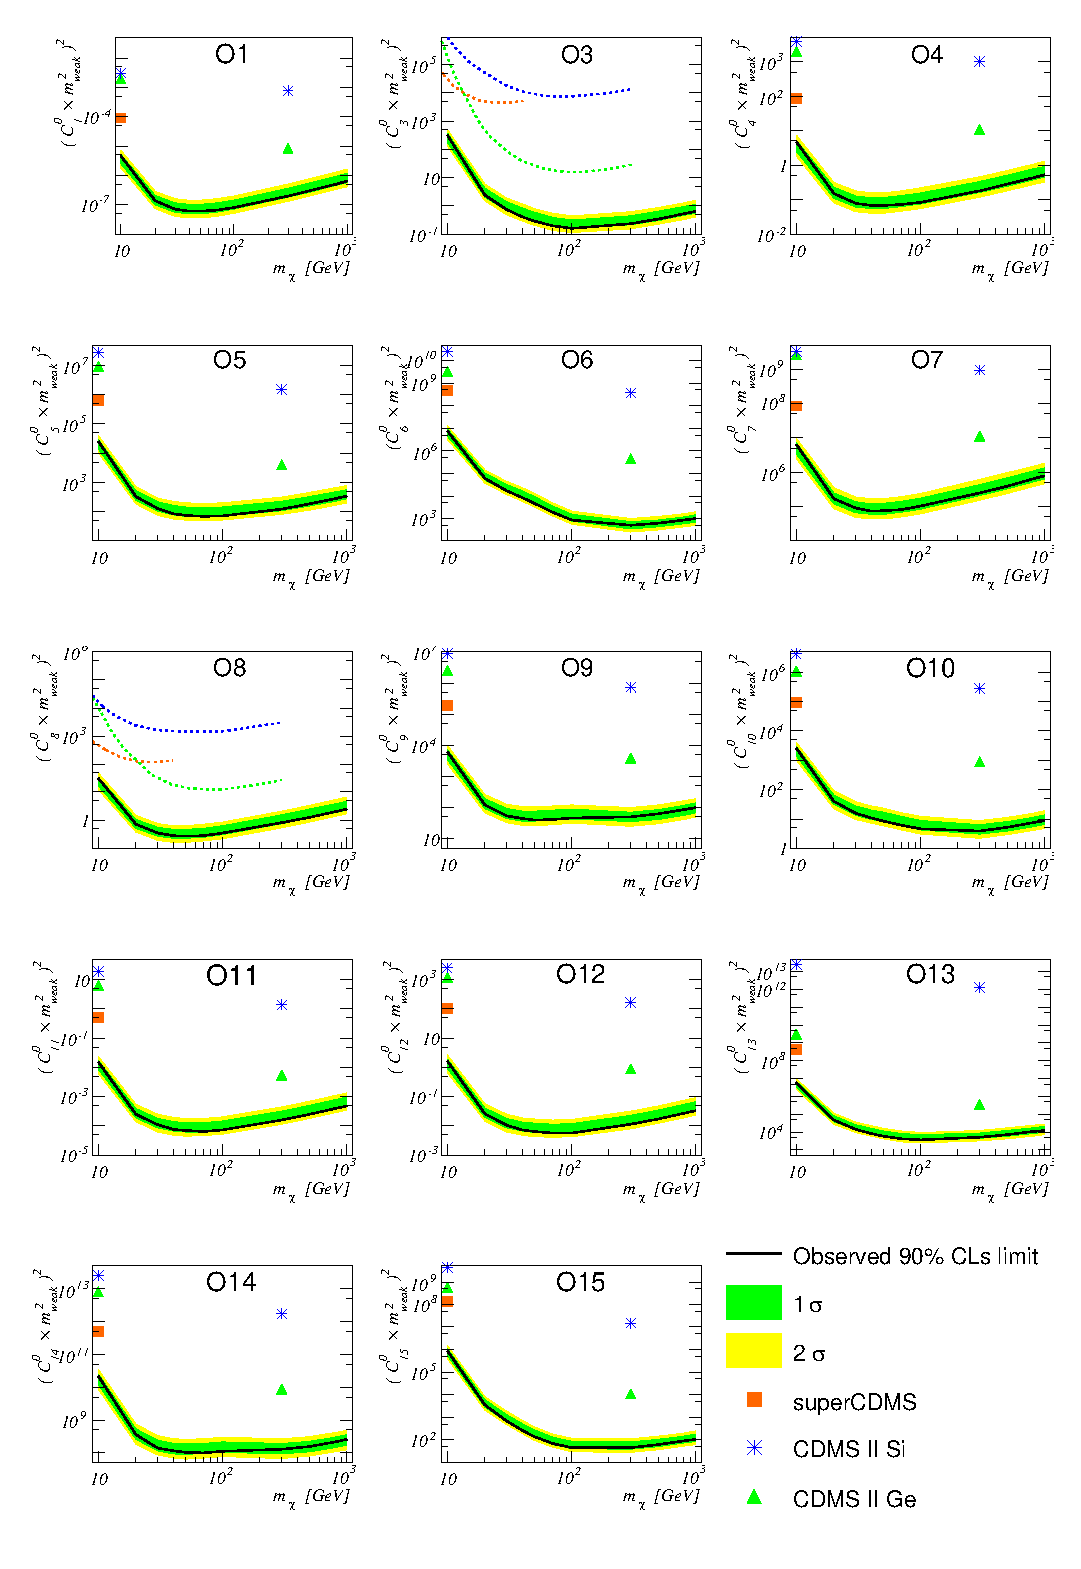
\includegraphics[width=\textwidth,height=\textheight,keepaspectratio]{Figures/ElasticAllLimitCDMS.eps}}
\end{minipage}
\caption{The \Xehund\ limits (90\% CL) Limits on isoscalar dimensionless coupling for all elastic scattering EFT operators are indicated in solid black. The expected sensitivity obtained assuming background only are is shown in green and yellow(1$\sigma$ and 2$\sigma$ respectively). Limits from CDMS-II Si CDMS-II Ge and SuperCDMS cite{CDMS} are presented in blue Astrix ,green triangle and orange rectangle (color online). For operator 3 and 8 a full limit from CDMS is published and is indicated by a dashed line in the respected colors.}
\label{fig:elasticLimit}
\end{figure*}


\subsection{Inelastic Scattering}

\begin{figure}[h!]
\centerline{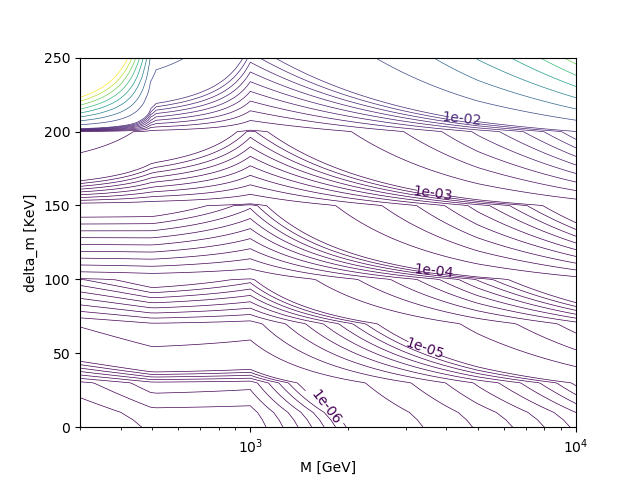
\includegraphics[width=1.\linewidth]{Figures/inelastic_delta_vs_m.png}}
\caption{90\% confidence level limits on coupling constant for $\mathcal{O}_1$ reported as a function of the WIMP mass and mass splitting $\delta$.}
\label{fig:2D_delta_vs_m}
\end{figure}  



\begin{figure*}
\begin{minipage}{1.\linewidth}
\centerline{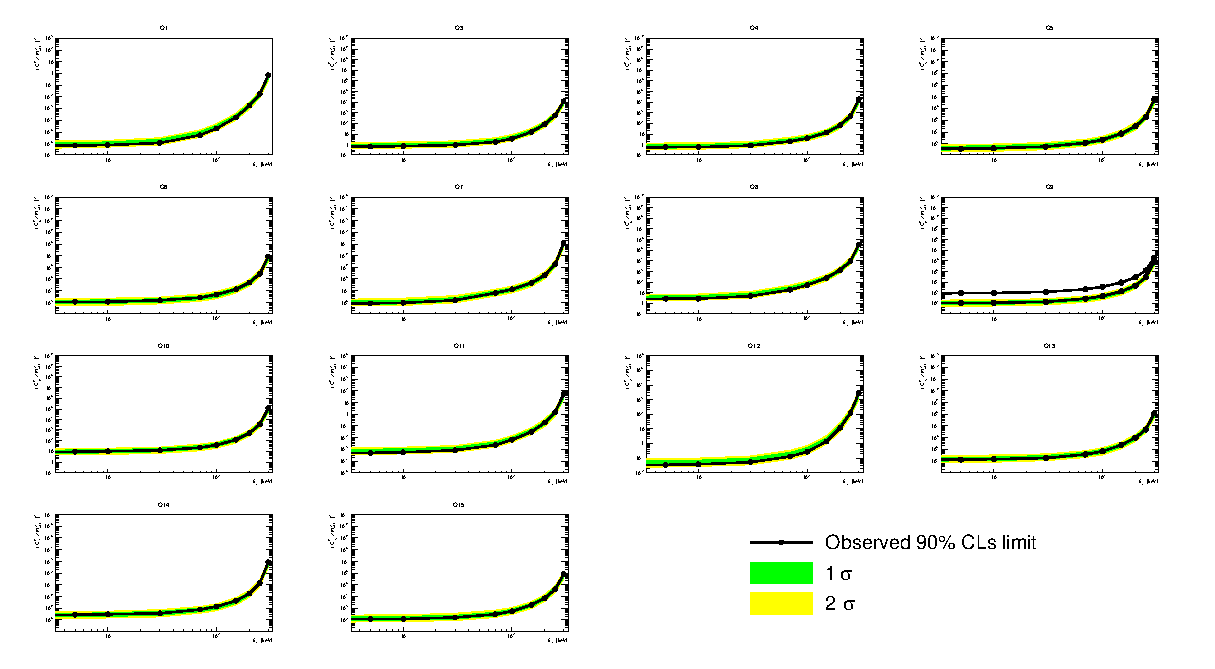
\includegraphics[width=1.\linewidth]{Figures/FinalInelastic.eps}}
\end{minipage}
\caption{The \Xehund\ limits (90\% CL) Limits on a 1 TeV/$c^2$ WIMP isoscalar dimensionless coupling for all inelastic scattering EFT operators are indicated in solid black. The expected sensitivity obtained assuming background only are is shown in green and yellow(1$\sigma$ and 2$\sigma$ respectively). }
\label{fig:elasticLimit}
\end{figure*}

\FloatBarrier

